\documentclass[%
aip,
jmp,
reprint,
floatfix
]{revtex4-1}

\usepackage{graphicx}% Include figure files
\usepackage{dcolumn}% Align table columns on decimal point
\usepackage{bm}% bold math
\usepackage{float}
\usepackage{siunitx}
\usepackage{hyperref}
\usepackage{listings}
\usepackage[english]{babel}
%\usepackage[backend=biber]{biblatex}
\usepackage[utf8]{inputenc}
%\addbibresource{refs.bib}
\usepackage{ gensymb }
%\usepackage[mathlines]{lineno}% Enable numbering of text and display math
%\linenumbers\relax % Commence numbering lines
\usepackage{color}
\usepackage{subcaption}

\definecolor{dkgreen}{rgb}{0,0.6,0}
\definecolor{gray}{rgb}{0.5,0.5,0.5}
\definecolor{mauve}{rgb}{0.58,0,0.82}

\lstset{
	frame=single, 
	language=Python, 
	columns=flexible,
	basicstyle={\footnotesize\ttfamily},
	keywordstyle=\color{blue},
	commentstyle=\color{dkgreen},
	stringstyle=\color{red},
	title=\lstname
}


\renewcommand{\arraystretch}{1.3} % Changes the height of tables
\DeclareSIUnit\year{yr}
\DeclareSIUnit\parsec{pc}



\begin{document}

	\title[Applying Coordinates to M29]{Applying Coordinates to M29}

	\author{Lucas, Miles}
	\author{Brandon, John}
	\affiliation{Iowa State University Department of Physics and Astronomy}

	\date{\today}


% Write here a short abstract (1 paragraph) describing what you achieved in this lab.

	\begin{abstract}

	\end{abstract}

	\maketitle
%________________________________________________________________________

%	Write here a summary of the goals of this lab. Be brief – do not exceed the end of the first page.

	\section{Introduction}

	

%________________________________________________________________________

%	Describe your telescope and camera setup. For the first lab you should describe the setup in more details. Subsequent labs can refer to the procedure described in the first lab, and focus more on the data acquisition itself. Important details to write include: which stars have been observed, which filters were used (BVI), what exposure times and what calibration procedures have been followed (e.g., dark frames acquisition, photometric standards observed, etc.). Mention also the observing conditions (weather, moon presence, temperature, etc.). You should include the observing log appendix A (a table or a scan of a hardcopy). This section can be as long as necessary, but you should strive for brevity (you can refer to the lab guide to avoid repeating all steps, but make sure you explain anything you did differently, problems encountered, etc.). Use tables to summarize information clearly.

	\section{Data Acquisition and Setup}
	Observations were made on \date{06 September 2017} at the Zaffarano Hall observation deck in Ames, Iowa (\ang{-93.64734}, \ang{42.02996}, \SI{342}{\meter}). The night was mostly clear and the ambient temperature was around \SI{12}{\degreeCelsius}. The moon was waning that night and had little to no effect on our sight. Observations were made using a Meade 8" reflector telescope with an SBIG ST-402ME CCD camera with internal V, B, and I filters. 
	
	Setting up the telescope was the same as previous observations made with the 8" Meade telescope at Zaffarano Hall.

%________________________________________________________________________

%Describe what you did to analyze the data. For the first lab this section will be minimal. For subsequent labs you should describe in detail the steps you did to analyze the data.  If applicable you can attach the code you used to analyze the data in Appendix B (either a log of your IDL section, or the code of any scripts you wrote). You can also attach screenshots of your computer session if it helps your discussion. Include tables of raw data in this section. The goal of this section is to describe unambiguously what you did to derive your final images and measured quantities from the raw data. Again be brief but complete (use as much space as you need).
	\section{Data Analysis}
	
	\begin{figure*}[t]
		\centering
		\begin{subfigure}[]{.45\textwidth}
			\centering
			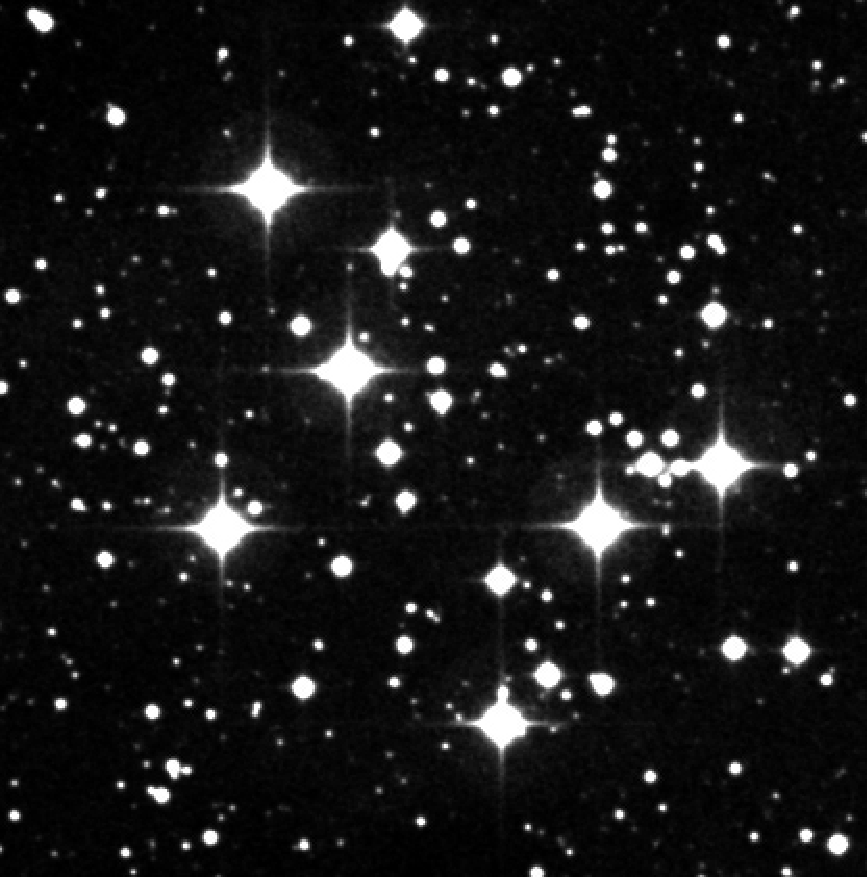
\includegraphics[width=\textwidth]{figs/dss.pdf}
		\end{subfigure}
		\qquad
		\begin{subfigure}[]{.45\textwidth}
			\centering
			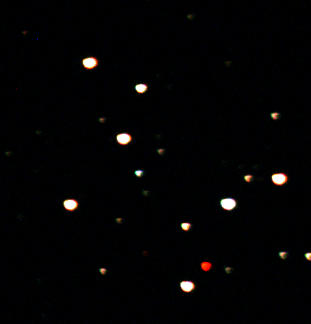
\includegraphics[width=\textwidth]{figs/rgb.pdf}
		\end{subfigure}
		\caption{dss vs us}
		\label{fig:map}
	\end{figure*}

%________________________________________________________________________

%	Describe in detail the results you obtained from the quantitative analysis of your data, as explained in the lab guide.
	\section{Results}

	

%________________________________________________________________________

%	Add here anything else you want to say, and summarize your results. This section should be very brief, not more than a couple of paragraphs
	\section{Conclusions}
	
	

%________________________________________________________________________

	\section*{Acknowledgments}

	Thank you to Dr. Charles Kerton and Brandon Marshall for their guidance and assistance in this work.

%	\printbibliography


%________________________________________________________________________

	\onecolumngrid
	\appendix
	\section{Observation Log}

	\begin{table}[H]
		\centering
		\caption{Observed 06 September 2017 by Miles Lucas and John Brandon}
\begin{tabular}{clclcccl}
	\hline
	Time  & File                   & N Frames & Object                                     & Filter &     Exposure     &       Camera Temp.        & Notes       \\ \hline\hline
	21:39 & M39\_2\_V\_13s\_       &    5     & M39 Objects x1, x4, x7, and x9; stars E, D &   V    & \SI{13}{\second} & \SI{5.33}{\degreeCelsius} &             \\
	21:41 & M39\_2\_V\_13s\_dark\_ &    5     & M39 Objects x1, x4, x7, and x9; stars E, D &   V    & \SI{13}{\second} & \SI{5.33}{\degreeCelsius} & Dark frames \\
	21:43 & M39\_2\_B\_13s\_       &    5     & M39 Objects x1, x4, x7, and x9; stars E, D &   B    & \SI{13}{\second} & \SI{5.33}{\degreeCelsius} &             \\ \hline
\end{tabular}

		\label{table:log}
	\end{table}
	
	
	

	

	\section{Catalog Analysis}

	\begin{figure}[H]
		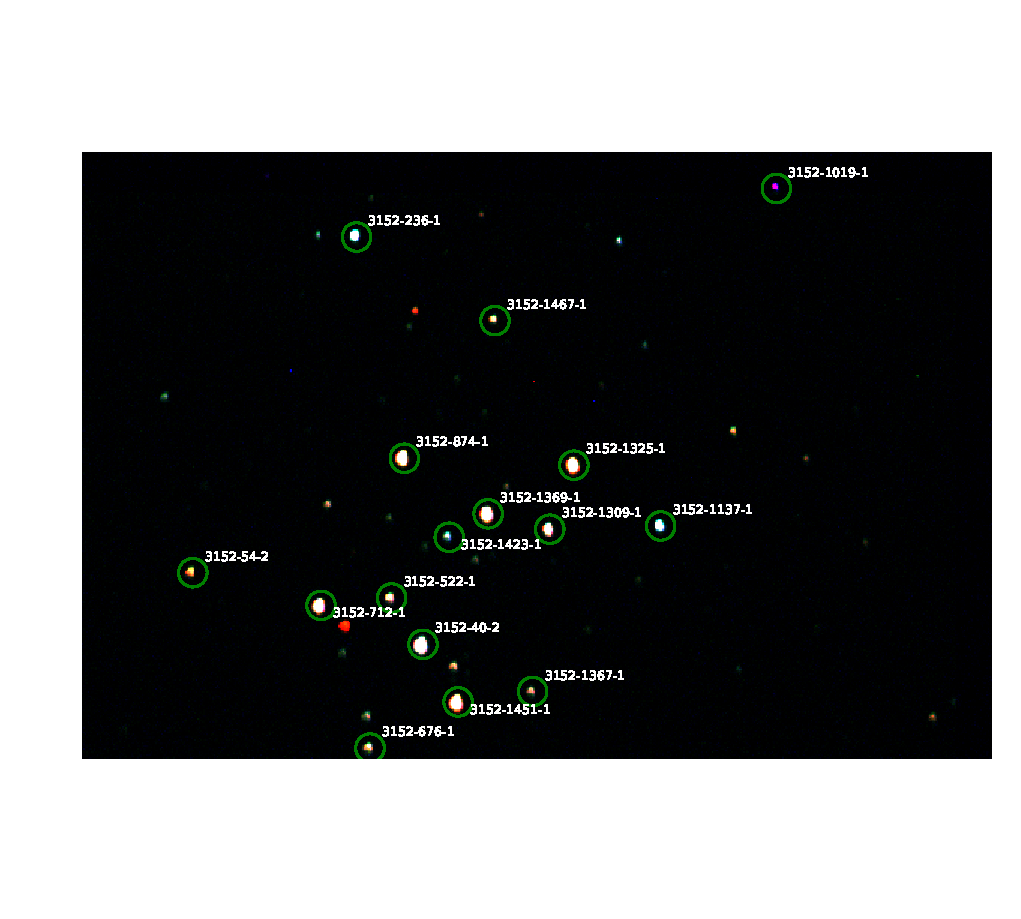
\includegraphics[]{figs/map.pdf}
	\end{figure}

	\section{Analysis Scripts}
	Also see Jupyter Notebook at \href{https://github.com/mileslucas/astro344l/blob/master/lab4/src/lab4.ipynb}{this Github page}.
	\lstinputlisting[label={lst:measurement}]{../src/imscale.py}
	
	

\end{document}
